\chapter{Experiments}

\section{Implementation}
The implementation of this work is done in \textit{Matlab} and it
is structured into multiple sections and files, to increase the modularity and 
readability of the code while simplifying the debugging process at the same time. 
The entire code is divided into the following categories:
\begin{itemize}
    \item A folder containing the \textbf{RLS} algorithm in the case where the sources
    do not influence one another;
    \item A folder containing the complete \textbf{PSO} algorithm integrated with 
    the PID control (the main focus of our work);
    \item A file with the complete \textbf{NSS} analysis of rotational invariance
    and symmetry properties;
    \item A file with the \textbf{PID} control applied to tracking the initial trajectory
    the drones follow for setup.
\end{itemize}
Th latter contains the same controller and model functions of the \texttt{Controller}
class of the PSO algorithm. The only difference consists in the desired velocities and positions, 
which are given by a predefined trajectory and by the PSO algorithm
respectively.

\noindent\\
The complete PSO with Control algorithm has the following main components: 
\begin{itemize}
    \item Setup and \textbf{\texttt{main loop}} of the simulation;
    \item The \textbf{\texttt{Particle}} class;
    \item The \textbf{\texttt{Controller}} class;
    \item The \textbf{\texttt{ARTVAs}} class;
    \item The \textbf{\texttt{Plotter}} class.
\end{itemize}
The main structure of the simulation is the following: 
we first perform a setup step in which we initialize the drones, 
the transmitting ARTVAs and other useful variables and constants.
Then, the simulation is divided into two phases:
\begin{itemize}
    \item \textbf{Exploration} phase: the drones are asked to position 
    themselves uniformly in the search space by followying a
    predifined trajectory;
    \item \textbf{Exploitation} phase: the drones are moved by the modified complete
    PSO algorithm to localive the multiple avalanche victims (ARTVAs).
\end{itemize}
If we have successfully estimated the position of all 
the trasmitting ARTVAs we stop the simulation, otherwise if any of the 
victims cannot be found the simulation stops after
a predefined (\texttt{n\_iterations}) maximum number of iterations.

\noindent\\
The implementation begings with the set-up of 
many variables and constants that will be useful throughout 
the whole experiment; and the initialization of the classes and theirs
crucial parameters (UAV physical quantities, controller gains and 
particles' data).
The most important hyperparameters 
include the number of drones (\texttt{n\_drones}), 
the number of iterations (\texttt{n\_iterations}), 
search space boundaries (\texttt{bounds}), 
and maximum velocity (\texttt{max\_velocity} or $v_\text{max}$). 
The sources (\texttt{p\_sources}) are fixed at predefined positions, 
and their number (\texttt{n\_sources}) determines how the drones are grouped 
during initialization, therefore 
we suppose we have at least a prior knowledge 
of the maximum number of victims. Instead, the PSO algorithm employs 
the inertia (\texttt{inertia} or $\omega$), cognitive (\texttt{cognitive\_factor} or $c_1$), 
and social (\texttt{social\_factor} or $c_2$) factors to 
balance exploration and exploitation, 
ensuring drones explore the search space efficiently
before converging to optimal solutions.
Other relevant parameters include the \texttt{velocity\_randomness} ($\beta$), 
which determines the level of percistency of excitation, the number of groups 
(\texttt{n\_groups}) which matches the number of sources and
the \texttt{communication\_radius} ($r_\text{comm}$), which sets the maximum range for drone 
data transfer.
Instead, the \texttt{step\_size} ($\alpha$) defines the meters the drones need to 
travel to move away from an exclusion zone they entered. 
The \texttt{exclusion\_zone\_radius} ($r_\text{excl}$) prevents redundant 
exploration near detected sources and avoids multiple drones 
converging on the same source. It is important in determining
the "resolution" of the algorithm, since no more than one victim can be found in that
radius by the drones, only by the human rescuers. 
A time step (\texttt{dt}) represents 
the $\tau_s$ control time, while the \texttt{iteration\_duration} 
is the $\Delta$ of 1 second in Section\ref{sec:PSO+PID}, determining the interval between one PSO 
update and another.
Each drone is has an initial position, velocity, and group affiliation, 
while a data structure is preallocated to store its trajectory 
throughout the search process.
In addition to this, we also initialize the \texttt{Plotter} class, 
whose job is to display in real time drone positions, trajectories, 
and exclusion zones in real time.

\noindent\\
Then the two phases begin:
the exploration phase uses a radial pattern to evenly partition 
the search space, dividing the space unfiformly 
between the drones. 
They move in straight lines toward their goals at maximum 
allowed speed. 

\noindent\\
Instead, during the main PSO loop, drones evaluate 
their positions based on the NSS signal received from the \texttt{ARTVAs} class. 
If a drone detects NSS values higher than a (\texttt{NSS\_threshold}),
it flags the localization of a drone.
Drones that enter exclusion zones move away from it and 
create a new group, with their velocities, 
personal best (\texttt{p\_best} or $\mathbf{pbest}$), and group best 
(\texttt{g\_best} or $\mathbf{gbest}$) resetted.

\noindent\\
After the real time simulation stops visualizing the final 
positions of drones and sources, plotting their trajectories, 
and computing errors between detected and true source positions. 

\subsection{\texttt{ARTVAs} class}
DA RIGUARDARE SE SI DECIDE DI CAMBIARE (M. OPPURE NO?)
The sole purpose of the \texttt{ARTVAs} class is to 
emit the signal received by a drone, the NSS. 
The signal is "emitted" using the \textit{send\_signal\_NSS()} 
function, which takes the position of the drone as 
input and returns a single floating-point value representing 
the perceived signal strength, the same in Eq.\ref{eq:final_model_more}.

\noindent\\
The main parameter of this class is \texttt{C}, a 
scaling factor that determines the magnitude of the NSS signals, 
whoch is set to a very high value of $10^8$, since we do not consider
the other physical parameters involved and the signal has very low values
with increasing distances.

\noindent\\
DA RIGUARDARE SE SI DECIDE DI CAMBIARE (M. OPPURE NO?)
It calculates both the combined signal strength 
from all sources and the individual contributions based 
on how far a drone is from each source. 
These calculations ensure that drones receive 
realistic signal strengths during the optimization process.
The \textit{superpositionNSS()} method computes the total 
NSS received by a drone by summing the signals from all sources, 
considering their distances from the drone. 
The \textit{send\_signal\_NSS()} method calculates the NSS from a
specific source to a given drone position. 
This is done using an inverse fourth-power relationship with distance, 
ensuring the signal weakens realistically 
as the drone moves farther from the source.
The \textit{send\_signal\_NSS()} method applies the formula 
described in Equation \ref{eq:distance_formula}, 
where \texttt{\(r\)} is capped at a minimum value of $10^{-5}$ 
to prevent division by zero. The NSS value is then calculated according 
to the formula in Equation \ref{eq:nss_formula}.

\subsection{\texttt{Plotter} class}
The \texttt{Plotter} class is the component that is responsible 
for the visualization of the simulation in real time during: 
it opens a separate window at the beginning
of the simulation and efficiently displays the simulation inside it.
It also provides methods for initializing plots, updating drone positions, 
displaying exclusion zones, and presenting trajectories. 
This visualization aids in monitoring the algorithm's 
progress and understanding group dynamics.
This class naturally includes properties to manage 
the figure sizes, axes limits, drone and source markers, color schemes, 
legends, and bounds of the plot.
It also updates the plot title with the current iteration 
number and simulation time.

\noindent\\
The \textit{draw()} method dynamically updates the positions of the 
drones and displays the fixed sources positions.
Since the draw calls of the \texttt{Plotter} can be the real bottleneck in the 
main loop of the simulation, we carefully optimized the code relative 
to this task so that redrawing the scene only updates the parts that 
changed between subsequent time-steps and everything else is kept as is.\\
Note that the simulation waits a defined time-step at each loop, 
from which all the computational time is subtracted, so to have faster simulations. 
However, this does not affect the time used to comment the results or for other 
calculations used in the algorithm, which remains the actual time it takes the 
drones to localize the victims. After this optimization, 
we managed to make the \texttt{Plotter} run fast 
enough that the simulation seems effectively in real time (since 
the draw calls do not run in a separate thread and therefore are blocking calls).\\

\noindent
In particular, the \texttt{Plotter} displays:
\begin{itemize}
    \item The exploration phase trajectory lines in radial shape with respect to 
    a imaginary circular boundary; 
    \item The drones, each assigned their own unique color based on their group affiliation;
    \item The positions of the real ARTVAs; 
    \item The position of the multiple estimations of the ARTVA, each with 
    the same color of the corresponding group;
    \item The exclusion zones, represented as circles whose centers are determined
    by the drone's position when the signals surpassed the threshold. 
\end{itemize}
Note that when a new group is created during 
the simulation, a new color is dynamically generated and added 
to the palette. The drone colors and the plot legend are updated 
accordingly.

\noindent\\
In the final stages of the simulation, the \textit{plot\_best()} 
method displays the best estimates for source positions achieved 
by each group. These estimates are marked with group-specific colors, 
and the legend is updated to include them. Similarly, 
the \textit{plot\_trajectories()} method visualizes the paths 
traveled by all drones, providing insight into their trajectories
during the PSO algorithm, since during the real-time simulation
the positions are shown only at each PSO time step $\tau_s$.

\subsection{\texttt{Controller} class}
\label{sec:controller_class}
The \texttt{Controller} class contains the 
complete quadrotor dynamics and the PID control laws. 
We define in it the physical properties of the drone, such as the mass, 
the inertia matrix, and the torque and drag coefficients.
Furthermore, we define the control proportional and derivative 
gains both for the $x$, $y$, $z$ positions and the 
the roll (\(\phi\)) and pitch (\(\theta\)) angles.

\noindent\\
The \textit{quadrotor\_full\_dynamics()} method computes 
the drone's translational and rotational dynamics based on 
its current state, external forces and torques. 
The state derivative is computed using the Equations\ref{eq:final_model_more}.

\noindent\\
A second method, \textit{control\_laws()}, is responsible 
for calculating the input force and torques required 
to control the quadrotor. This method first computes 
the position and velocity errors, which are used to 
determine the desired thrust like in Eq.~\ref{eq:desired_thrust}. 
From this desired thrust, the method calculates its 
$x$ and $y$ components \(T_x\) and \(T_y\), 
which are used to derive the desired roll \(\phi_d\) 
and pitch \(\theta_d\) angles with Eqs. \ref{eq:desire_phi}, 
\ref{eq:desire_theta} respectively. 
The desired yaw torque is computed separately 
to align the quadrotor with the desired heading, 
ensuring accurate orientation control. These desired angles and the 
associated angular velocity errors are then combined 
with the controller gains to calculate the commanding input torques,
following Eqs. \ref{eq:input_phi}, \ref{eq:input_theta}, 
\ref{eq:input_psi}. 

\noindent\\
Finally, the \textit{compute\_rotor\_velocities()} 
method determines the rotor speeds needed to achieve 
the commanding thrust and torques. The speeds are found 
inverting $\mathbf{A}$ matrix as in Eq.\ref{eq:rotor_velocities}.
The computed rotor speeds are checked 
to ensure non-negative values, as negative speeds are 
physically invalid.

\subsection{\texttt{Particle} class}
The \texttt{Particle} class, which is also called \texttt{Drone} 
class, models each drone in the conplete PSO algorithm integrated with the PID
control and postioning phase. 
\noindent\\
Each particle stores its current 
position and velocity, as well as its personal 
best position (\texttt{p\_best}), the corresponding
highest NSS value found so far (\texttt{nss\_best}), 
their group index (\texttt{group\_idx}), 
the \texttt{victim\_found\_flag} to remember the found source and 
data structures to remember the exclusion zones 
that have been shared with and by the drone.
The constructor of the class initializes the position 
at the center of the search space, and the personal best
to this position.

\noindent\\
This class contains the most important 
methods: the \textit{update\_velocity()} method modifies the 
particle's velocity using the formula described
in \ref{eq:model_velocity2}. Then, random noise is 
added to the velocity as in Eq.\ref{eq:persistence_of_excitation},
while constraints ensure the velocity does not 
exceed the \texttt{max\_velocity} following Eq. \ref{eq:velocity_clamping}.

\noindent\\
Instead, the \textit{update\_state()} function is the one responsible
of the implementation of the complete quadrotor dynamics
and control laws, by calling the respective methods we have seen 
in the \texttt{Controller} class\ref{sec:controller_class}.
This is achieved through the initialization of a \texttt{Controller}
class in every \texttt{Drone} class.

\noindent\\
Furthermore, the \textit{evaluate\_nss()} method calculates the 
NSS value at the particle's current position by passing the 
\texttt{ARTVAs} class approriate function, as described 
in Algorithm\ref{alg:evaluate_nss}.
Its personal best is updated if higher then the previous best. 
and if the particle discovers a source  
it sets the flag to create an exclusion zone to true.
The exclusion zone is mantained until the end 
of the simulation. 
In this last case the inertia is reduced to decrease 
the excitation level.
\SetKwFunction{Fdue}{\texttt{evaluate\_nss}}
\begin{algorithm}[h]
     \caption{\texttt{evaluate\_nss} (MATLAB function)}\label{alg:evaluate_nss}
     \KwIn{$\mathbf{p}_r$: current position of the particle.}
     \KwIn{\texttt{p\_sources}: array of source positions.}
     \KwIn{$superpositionNSS$: function to compute the total NSS at a given position.}
     \KwOut{\texttt{nss\_value}: NSS value at the particle's current position.}
     \KwOut{\texttt{p\_best}: personal best position.}
     \KwOut{\texttt{nss\_best}: personal best NSS value.}
     \KwOut{\texttt{my\_exclusion\_zone}: center of the created exclusion zone.}
     \vspace{0.3\baselineskip}
     \nonl \Fn(\tcc*[h]{}){\Fdue{$\mathbf{p}_r$, \texttt{p\_sources}}}{
        \SetAlgoBlockMarkers{}{}
        \DontPrintSemicolon \nonl \textbf{Compute the NSS value at the current position:}\;\PrintSemicolon
        \texttt{nss\_value} $\gets$ \textit{superpositionNSS}($\mathbf{p}_r$, \texttt{p\_sources})\;

        \If{ \texttt{nss\_value} $>$ \texttt{nss\_best}}{
            \texttt{p\_best}$ \gets \mathbf{p}_r$\;
            \texttt{nss\_best} $\gets$ \texttt{nss\_value}\;
        }
        \ElseIf{\texttt{nss\_value} $>$ \texttt{NSS\_threshold} \textbf{and} \texttt{victim\_found\_flag} = \texttt{false}}{
            \texttt{victim\_found\_flag} $\gets$ \texttt{true}\;
            \texttt{my\_exclusion\_zone} $\gets \mathbf{p}_r$\;
            \texttt{inertia} $\gets 0.5$\;
        }
     }
 \end{algorithm}

\noindent\\
Communication between particles is allowed only by the 
\textit{can\_I\_communicate\_with()} method, which 
determines if two particles are within the predifined 
communication radius, which is condition \ref{eq:in_comm}.

\noindent\\
The \textit{share\_exclusion\_zones()} 
method allows the drone to communicate to its 
neighbouring drones the position 
of the found "supposed" source.

\noindent\\
Finally, the
\textit{check\_if\_in\_exclusion\_zone()} 
method verifies if a particle is inside any 
exclusion zone the drones knows of and  
the \textit{move\_away\_from\_exclusion()} function
makes the drone take  big "jump" in the same incoming direction
to get as far as possible from the zone, the goal 
position is computed using Eq.\ref{eq:move_away}.

\subsection{\texttt{Main Loop}}
DECIDERE SE UNIFORARE LE VAR A TEXTTT MA POI NON ABBIAMO GLI 
STESSI NOMI DELLA PARTE TEORICA, QUINDI DECIDI IN TUTTI GLI ALG
The first step in the \texttt{main loop} involves the initialization
of the UAVs (particles) and in particular the sorting of 
the drones in different groups as described in Algorithm\ref{alg:sort_drones_in_groups}.
DESCRIVERE BREVEMENTE LA FUNZIONE UNA RIGA, DOPO CHE C E LA VERSIONE DEFINITIVA
ATTENZIONE QUESTA FUNZIONE ANDREBBE MODIFICATA ANCHE NEL CODICE
PERCH\`E A VOLTE NON FUNZIONA
\SetKwFunction{Funo}{\texttt{sort\_drones\_in\_groups}}
\begin{algorithm}[h]
    \caption{\texttt{sort\_drones\_in\_groups} (MATLAB function)}\label{alg:sort_drones_in_groups}
    \KwIn{\textbf{\texttt{n\_drones}}: number of drones available for assignment.}
    \KwIn{\textbf{\texttt{n\_sources}}: number of sources to which drones need to be assigned.}
    \KwOut{\textbf{\texttt{group\_indices}}: array of indices indicating the assigned group.}
    \KwOut{\textbf{\texttt{n\_groups}}: the obtained number of groups.}
    \vspace{0.3\baselineskip}
    \nonl \Fn(\tcc*[h]{}){\Funo{\texttt{n\_drones}, \texttt{n\_sources}}}{
    \SetAlgoBlockMarkers{}{}
    \If{\texttt{n\_drones} $>$ \texttt{n\_sources}}{
        \textbf{Assign} at least one drone to each group, following mathematical order\;
        \textbf{Assign randmly} remaining drones to existing groups\;
    }
    \ElseIf{\texttt{n\_drones} = \texttt{n\_sources}}{
        \textbf{Assign} each drone to a unique group\;
    }
    \Else{
        \textbf{Assign orderly} drones up to \texttt{n\_drones}\;
    }
    \textbf{Set} the number of groups: \texttt{n\_groups} $\gets \texttt{max(group\_indices)}$\;
    }
\end{algorithm}

\noindent Note that the function \texttt{sort\_drones\_in\_groups} ensures the creation of sufficient groups 
for the localization of multiple sources only when the number of drones is equal to or greater than 
the number of sources.

\subsection{Exploration phase}
At the start of the simulation, all drones are located at the origin of the search space.
During the first Exploration Phase, the PSO algorithm is not yet employed. 
During this phase, the drones move according to predefined trajectories at maximum speed $v_{\text{max}}$. 
The trajectories are determined based on the number of drones and follow a radial pattern, as shown in Figure \ref{fig:exploration_pattern}. 
The drones follow these trajectories until they have covered a distance \texttt{travel\_distance} equivalent to half the boundary of the search space.
The goal each drone needs to reach is computed using the following Algorithm~\ref{alg:exploration_goals}:
\SetKwFunction{Ftre}{\texttt{exploration\_goal}}
\newcommand{\forcond}{drone $j=1$ \KwTo $m$}
\begin{algorithm}[h]
    \caption{\texttt{exploration\_goal} (MATLAB function)}\label{alg:exploration_goals}
    \KwIn{\texttt{n\_drones}: number of drones available for exploration.}
    \KwIn{\texttt{bounds}: maximum limit of the search space.}
    \KwOut{\texttt{goals}: array containing $x$,$y$ positions of the exploration goals.}
    \vspace{0.3\baselineskip}
    \nonl \Fn(\tcc*[h]{}){\Ftre{\texttt{n\_drones}, \texttt{bounds}}}{
    \SetAlgoBlockMarkers{}{} \DontPrintSemicolon
    \KwInitialize{ an empty array \texttt{goals}.}\;
    \textbf{Set} \texttt{angle\_step} $\gets \frac{360}{\texttt{n\_drones}}$.\;
    \textbf{Set} \texttt{travel\_distance} $\gets \frac{\texttt{bounds}}{2}$.\;
    \PrintSemicolon
    \For{\forcond}{
        \textbf{Compute} angle for the current drone: \texttt{drone\_angle} $\gets j \cdot \texttt{angle\_step}$\;
        \textbf{Calculate} slope: \texttt{m} $\gets \tan(\textit{deg2rad}(\texttt{drone\_angle}))$\;
        \DontPrintSemicolon \tcc*[h]{\hfill 1st quadrant \hfill }\; \PrintSemicolon
        \uIf{\texttt{drone\_angle} $>$ 315 \textbf{or} \texttt{drone\_angle} $\leq$ 45}{
            \textbf{Set} \texttt{goal} $\gets [\texttt{travel\_distance}, \texttt{m} \cdot \texttt{travel\_distance}]$
        }
        \DontPrintSemicolon \tcc*[h]{\hfill 2nd quadrant \hfill }\; \PrintSemicolon
        \ElseIf{\texttt{drone\_angle} $>$ 45 \textbf{and} \texttt{drone\_angle} $\leq$ 135}{
            \textbf{Set} \texttt{goal} $\gets [\frac{\texttt{travel\_distance}}{\texttt{m}}, \texttt{travel\_distance}]$ 
        }
        \DontPrintSemicolon \tcc*[h]{\hfill 3rd quadrant \hfill }\; \PrintSemicolon
        \ElseIf{\texttt{drone\_angle} $>$ 135 \textbf{and} \texttt{drone\_angle} $\leq$ 225}{
            \textbf{Set} \texttt{goal} $\gets [-\texttt{travel\_distance}, \texttt{m} \cdot -\texttt{travel\_distance}]$ 
        }
        \DontPrintSemicolon \tcc*[h]{\hfill 4th quadrant \hfill }\; \PrintSemicolon
        \ElseIf{\texttt{drone\_angle} $>$ 225 \textbf{and} \texttt{drone\_angle} $\leq$ 315}{
            \textbf{Set} \texttt{goal} $\gets [-\frac{\texttt{travel\_distance}}{\texttt{m}}, -\texttt{travel\_distance}]$ 
        }
        \texttt{goals} $\gets$ \texttt{goals} + [\texttt{goal}]\;
    }
    }
\end{algorithm}

\noindent
where \texttt{angle\_step} is the angular increment to uniformly divide the space,
\texttt{drone\_angle} represents the angle assigned to each drone, 
while \texttt{m} is the slope of the trajectory calculated from the drone's angle. 

\begin{figure}
    \centering
    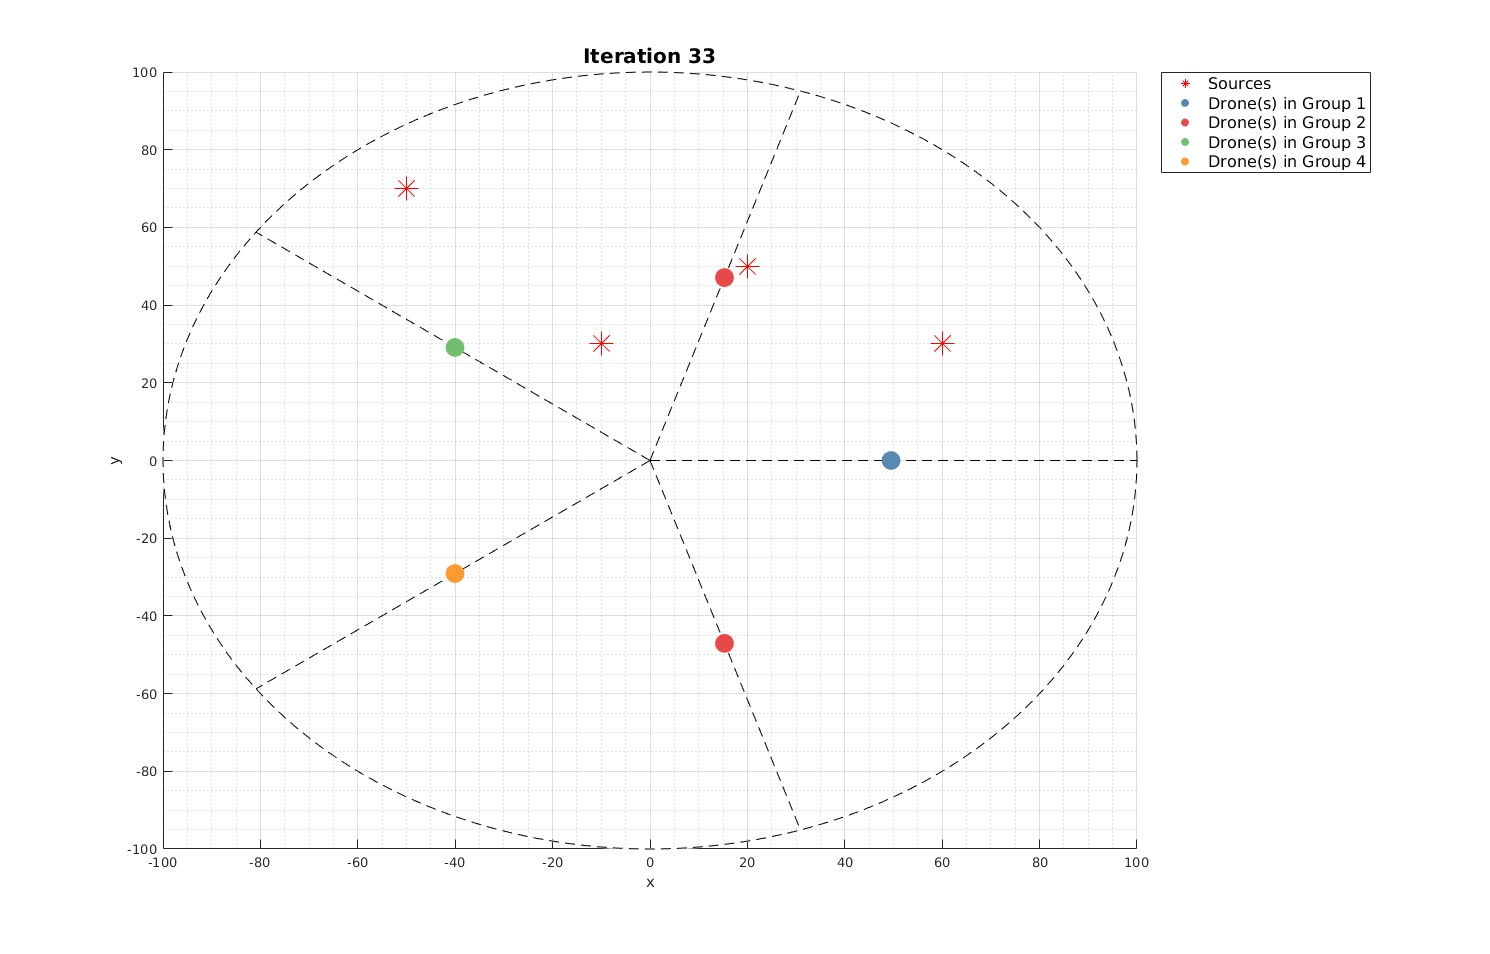
\includegraphics[width=\textwidth]{images/exploration_pattern.jpg} 
    \caption{Radial exploration pattern for 5 drones at the end of the Exploration Phase.}
    \label{fig:exploration_pattern}
\end{figure}

\subsubsection{Exploitation Phase}
This is the most important part of the simulation since it involves
the localization of the victims through the deployment of our modified PSO
algorithm with the PID control, described in Section \ref{sec:PSO+PID}.

\noindent\\
At each $\tau_s$ iteration step until \texttt{n\_iterations},
each $j$-th UAV checks the neighbouring drones with the
\textit{can\_I\_communicate\_with()} function and with a 
positive response they share their exclusion zones with each other
(if they have found a source). The communication radio (\(r_{\text{comm}}\))
is set to 10\,m.

\noindent\\
Then, it calls \textit{check\_if\_in\_exclusion\_zone()}
to verify if it's position is inside the radius of any of the 
saved exclusion zones.
In case of a positive response, the drone is commanded to 
execute the \textit{move\_away\_from\_exclusion()} function. 
Then, its velocity is reset to zero, and its personal 
best position, \texttt{p\_best}, is assigned to a random point 
far from the new location. Additionally, the $\mathbf{gbest}$ 
is reset to \(-\infty\), and the 
drone's \texttt{nss\_best} is also reset to \(-\infty\), 
ensuring the drone restart exploring with a fresh start.
DOBBIAMO DIRE CHE TRASFERIMENTO È INSTANTANEO?
DECIDERE SE DIRLA QUESTA COSA O IMPLEMENTARE LA COSA FATTA BENE:
For simplicity reasons, this movement is considered "instantaneous", 
meaning that in the simulation, the drone's journey to the goal is 
not displayed. Instead, in the next iteration, it will already 
be at the designated location. However, the number of 
iterations and the simulation time account for the actual 
time required for the drone to reach the goal at maximum speed.
In case of a negative response, the \textit{evaluate\_nss()} is 
called and the group best ($\mathbf{gbest}$) is updated if the received NSS signal 
is greater than the previous best.
\SetAlgoBlockMarkers{}{}
\begin{algorithm}[h!]
    \DontPrintSemicolon
    \caption{Particle Swarm Optimization for Multi-Source Localization}\label{alg:PSO}
    \KwInitialize{positions of drones to the center of the search space.}\;
    \KwInitialize{\texttt{g\_best\_values}.}\;
    \textbf{Assign} each drone to a group using the function in Algorithm \ref{alg:sort_drones_in_groups}.\;
    \vspace{0.3\baselineskip}
    \DontPrintSemicolon \nonl \textbf{Exploration Phase:}\; \PrintSemicolon
    \textbf{Compute} exploration goals using the function in Algorithm \ref{alg:exploration_goals}\;
    \For{\forcond}{
        \textbf{Move} to goal with \texttt{max\_velocity}\;
    }
    \vspace{0.3\baselineskip}
    \DontPrintSemicolon \nonl \textbf{Exploitation Phase:}\; \PrintSemicolon
    \For{\( \tau_s = 1 \) to \texttt{n\_iterations}}{
        \For{\forcond}{
            \For{\textbf{each} other drone \(l \neq j\)}{
                \If{\textit{can\_I\_communicate\_with()} \textbf{or} \texttt{victim\_found\_flag} = \text{true}}{
                    \textbf{Share} exclusion zones between \(j\) and \(l\)\;
                }
            }
            
            \If{\textit{check\_if\_in\_exclusion\_zone()} = true}{
                \If{\textbf{drone} \(j\) is not alone in its group}{
                    \textbf{Reassign} drone \(j\) to a new group\;
                    \textbf{Initialize} new \texttt{g\_best} and \texttt{nss\_best}\;
                }
                \textbf{Move} away from exclusion zones\;
                \textbf{Reset} personal best \texttt{p\_best}\;
                \textbf{Set} drone \(j\) \texttt{inertia} to 0.5\;
            }
            \Else{
                \textbf{Evaluate} NSS at \(\mathbf{p}_j(\tau_s)\)\;
                \If{\texttt{nss\_value} \( > \) \texttt{nss\_best}}{
                    \textbf{Update} \texttt{p\_best}\;
                }
                \If{\texttt{nss\_value} \( > \) \texttt{g\_best}}{
                    \textbf{Update} \texttt{g\_best\_values}\;
                }
            }
            \textbf{Compute} desired velocity: \textit{update\_velocity()}\;
            \textbf{Apply} persistence of excitation as in Eq.\eqref{eq:persistence_of_excitation}\;
            \textbf{Limit} velocity to \texttt{max\_velocity} as in Eq.\eqref{eq:velocity_clamping}\;
            \textbf{Desired} position: as in Eq.\eqref{eq:model_position2}\;
            \textbf{Set} \texttt{iteration\_duration} to 1\;
            \For{\(\texttt{t} = 0 : \texttt{dt} : \texttt{iteration\_duration}\)}{
                \textbf{Control} dynamics: \textit{update\_state()}\;
                \textbf{Enforce} boundaries on position as in Eq.\eqref{eq:boundary_condition}\;
            }
        }
    }
\end{algorithm}    

\noindent\\
Subsequently, the \textit{update\_velocity()} method computes the desired 
velocity command for the control loop and the desired position is obtained 
using the standard PSO formula in Eq. \ref{eq:model_position2}.
At each time step $\tau_k$ until the end of the $\Delta$, 
the \textit{update\_state()} function is called and the
boundries are enforced as in \ref{eq:boundary_condition}.
Finally, we can present the complete modified PSO algorithm in 
Algorithm \ref{alg:PSO}: 

Note that the inertia of a drone that has found a source 
is set to zero (\(\omega = 0\)), increasing
convergence speed. The final output is the set of best estimates 
\texttt{g\_best\_values}, composed of the best estimated position 
of a source by each group.

\newpage
\section{Results}
METTERE UNA FOTO VOLENDO
SPOSTARLI TUTTI SOPRA

The parameters relative to the UAVs physical
characteristics used in the simulations are from 
the real Dragonfly IV drone \cite{drone}, these values are
summarized in Table\ref{tab:drone_parameters}.
In both experiments (trajectory tracking and PSO with
control) these same parameters are used for the control
part, in conjunction with the gains 
described in Table~\ref{tab:control_gains}.
\begin{table}[h!]
\centering
\caption{Drone Parameters for PSO and Trajectory Tracking Control}
\begin{tabular}{|l|c|l|}
\hline
\textbf{Parameter}           & \textbf{Symbol}  & \textbf{Value} \\ \hline
Mass                        & \(m\)           & \(0.4 \, \text{kg}\) \\ \hline
Moment of inertia (x-axis)  & \(J_x\)         & \(3.8278 \times 10^{-3} \, \text{kg}\,\text{m}^2\) \\ \hline
Moment of inertia (y-axis)  & \(J_y\)         & \(3.8278 \times 10^{-3} \, \text{kg}\,\text{m}^2\) \\ \hline
Moment of inertia (z-axis)  & \(J_z\)         & \(7.1345 \times 10^{-3} \, \text{kg}\,\text{m}^2\) \\ \hline
Arm length                  & \(l\)           & \(0.205 \, \text{m}\) \\ \hline
Thrust coefficient          & \(c_t\)         & \(6.354 \times 10^{-4}\) \\ \hline
Torque coefficient          & \(c_d\)         & \(0.048\) \\ \hline
\end{tabular}
\label{tab:drone_parameters}
\end{table}
\begin{table}[h!]
\centering
\caption{Control Gain Values}
\label{tab:control_gains}
\begin{tabular}{|c|c|c|}
\hline
\textbf{Control Type} & \textbf{Proportional Gain} & \textbf{Derivative Gain} \\ \hline
Position Control (\(x\)) & \(k_{xp} = 0.1\)         & \(k_{xd} = 0.5\)         \\ \hline
Position Control (\(y\)) & \(k_{yp} = 0.1\)         & \(k_{yd} = 0.54\)        \\ \hline
Position Control (\(z\)) & \(k_{zp} = 1.0\)         & \(k_{zd} = 2.5\)         \\ \hline
Attitude Control (\(\phi\)) & \(k_{p\phi} = 2.0\)     & \(k_{d\phi} = 2.5\)      \\ \hline
Attitude Control (\(\theta\)) & \(k_{p\theta} = 2.0\)  & \(k_{d\theta} = 2.5\)    \\ \hline
Attitude Control (\(\psi\)) & \(k_{p\psi} = 2.0\)     & \(k_{d\psi} = 4.0\)      \\ \hline
\end{tabular}
\end{table}
\noindent\\
Instead, the hyperparameters relative to the PSO algorithm are
defined in Table \ref{tab:pso_parameters}.
\begin{table}[h!]
\centering
\caption{PSO Hyperparameters and Settings}
\begin{tabular}{|l|c|c|}
\hline
\textbf{Parameter}            & \textbf{Symbol}         & \textbf{Value} \\ \hline
Number of drones             & \(n_{\text{drones}}\)   & 4 \\ \hline
Number of iterations         & \(n_{\text{iterations}}\) & 310 \\ \hline
Search space bounds          & \(\text{bounds}\)       & \([-80, 80]\) \\ \hline
Maximum velocity             & \(v_{\text{max}}\)      & 2 \\ \hline
Source positions             & \(p_{\text{sources}}\)  & \([20, 50], [-50, 70], [60, 30], [-10, 30]\) \\ \hline
Number of sources            & \(n_{\text{sources}}\)  & 4 \\ \hline
Inertia weight               & \(w\)                  & 1.05 \\ \hline
Cognitive factor             & \(c_{\text{cognitive}}\) & 2.05 \\ \hline
Social factor                & \(c_{\text{social}}\)   & 1.5 \\ \hline
Velocity randomness          & \(r_v\)                & 0.6 \\ \hline
Communication radius         & \(r_{\text{comm}}\)     & 10 \\ \hline
Step size                    & \(s\)                  & 90 \\ \hline
Exclusion zone radius        & \(r_{\text{excl}}\)     & 3 \\ \hline
Time step                    & \(\Delta t\)           & 0.04 \\ \hline
Iteration duration           & \(t_{\text{iter}}\)     & 1 \\ \hline
\end{tabular}
\label{tab:pso_parameters}
\end{table}
\noindent\\
Each drone in the Particle Swarm Optimization (PSO) framework is 
initialized with a set of carefully chosen parameters. 
The drones start their search with an initial position at the 
center of the search space, defined as \([0, 0]\). 
Their initial velocities are randomized using a scaling factor of \(0.6\), 
which adds variation, and capped at a maximum velocity of \(2 \, \text{m/s}\) 
to prevent overshooting targets. The search space is constrained within bounds 
of \([-80, 80]\) for both the x and y directions.

Each drone's best-known position (\(p_{\text{best}}\)) is initialized 
to its starting position, while its best Normalized Source Strength (NSS) 
value is set to \(-\infty\), ensuring that any detected signal improves 
its current state. The drones operate with an inertia weight of \(1.05\), 
balancing exploration and exploitation during the optimization process. 
Additionally, an exclusion zone radius of \(3 \, \text{m}\) is defined, 
representing a region where the NSS signal diminishes significantly.

The drones are grouped based on a variable group index, allowing for 
clustering when searching for multiple targets. Each drone also has a 
specific goal position that acts as its target during the optimization process. 
For orientation and dynamics, the roll, pitch, and yaw angles (\(RPY\)) 
are initialized to \([0, 0, 0]\), ensuring a neutral starting orientation. 
These parameters collectively define the initial state and behavior of the 
drones in the PSO framework.


In the context of search and rescue (S\&R) missions, the number of available 
UAVs is typically limited (ranging from 1 to 10 \cite{PSO_original}), and 
the search area 
usually spans only a few thousand square meters.
Therefore, it is reasonable to 
assume the presence of a communication network with a static topology, allowing 
for the implementation of a centralized estimation algorithm.

\subsection{PID for Trajectory Tracking}
METTERE LA TRAIETTORIA CHE VIENE SEGUITA
The results of PID control using the full quadrotor dynamics 
model \eqref{eq:final_model},
applied to trajectory tracking during the first positioning 
(exploration) phase of the algorithm, 
are presented in the following figures: 
Figure \ref{fig:pd_traj_comparison} illustrates 
the comparison between the actual and desired trajectory in 3D space, 
showcasing the effectiveness of the control strategy in 
aligning the drone's path with the desired trajectory. 
Figures \ref{fig:pid_x}, \ref{fig:pid_y}, and \ref{fig:pid_z}
provide a detailed breakdown of the trajectory t
racking along the \(x\), \(y\), and \(z\) axes, respectively. 
These plots highlight the individual tracking performance 
in each dimension and confirm the controller's precision 
in following the desired positions.

Figure \ref{fig:pid_sim} shows the simulation over time,
providing an overview of the control system's behavior 
during this phase. Additionally, the rotor velocities 
calculated using \eqref{eq:rotor_velocities} are plotted 
in Figure \ref{fig:rotor_velocities}. This figure provides 
insights into the actuation required to achieve the desired 
trajectory.

\begin{figure}[h!]
    \centering
    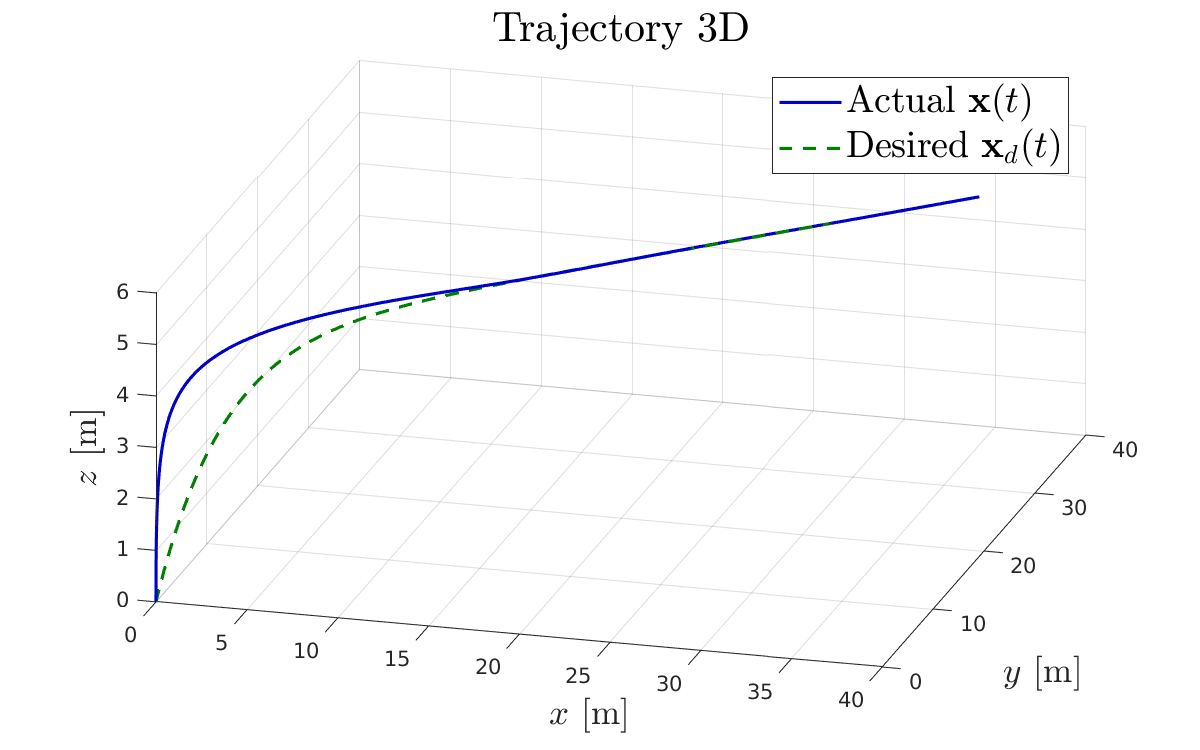
\includegraphics[width=1\textwidth]{images/traj_comparison.png}
    \caption[3D Trajectory Tracking]{Comparison of the actual and desired trajectory in 3D space during the exploration phase.}
    \label{fig:pd_traj_comparison}
\end{figure}

\begin{figure}[h!]
    \centering
    \begin{minipage}[b]{0.49\textwidth}
        \centering
        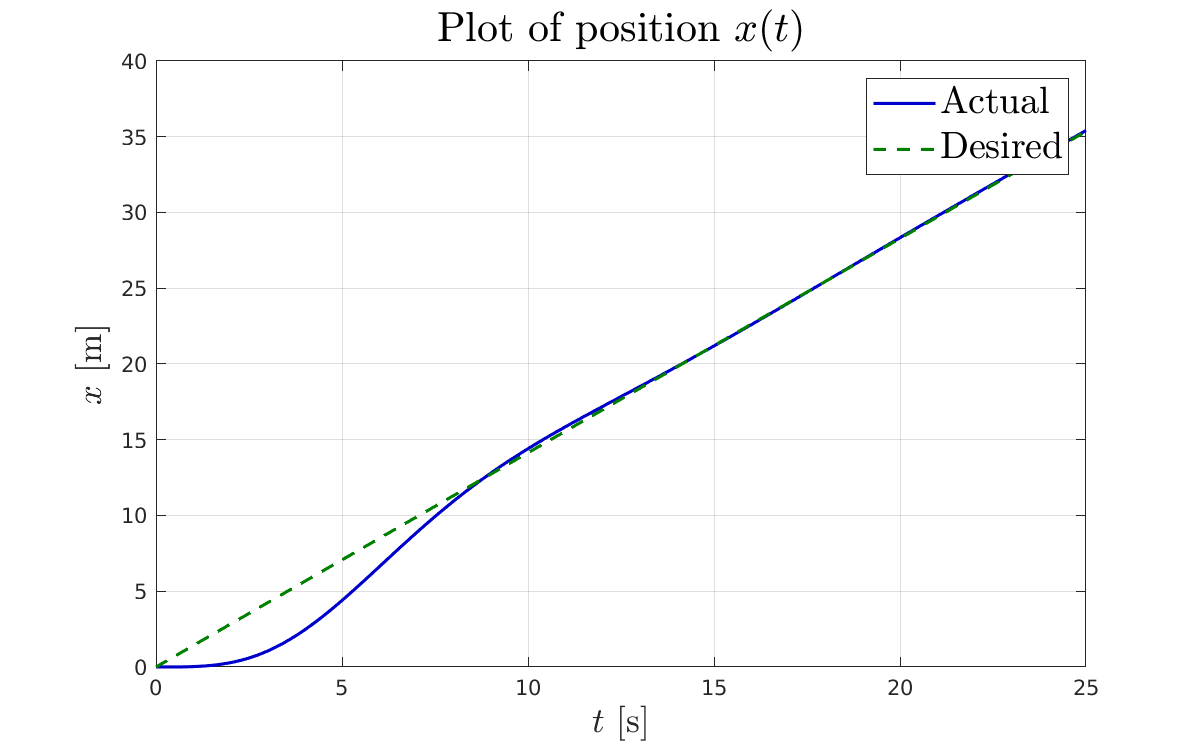
\includegraphics[width=\textwidth]{images/pid_x.png}
        \caption[Tracking in X-axis]{Actual and desired $x$ position over time.}
        \label{fig:pid_x}
    \end{minipage}
    \begin{minipage}[b]{0.49\textwidth}
        \centering
        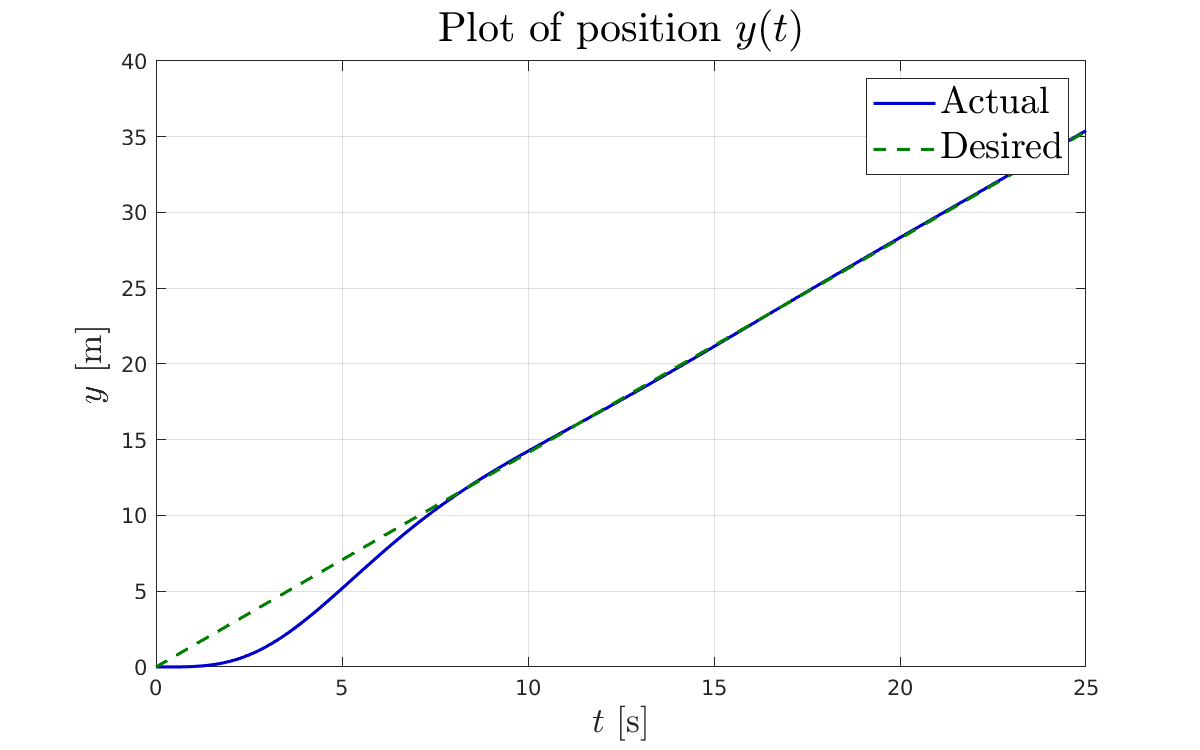
\includegraphics[width=\textwidth]{images/pid_y.png}
        \caption[Tracking in Y-axis]{Actual and desired $y$ position over time.}
        \label{fig:pid_y}
    \end{minipage}
    \begin{minipage}[b]{0.49\textwidth}
        \centering
        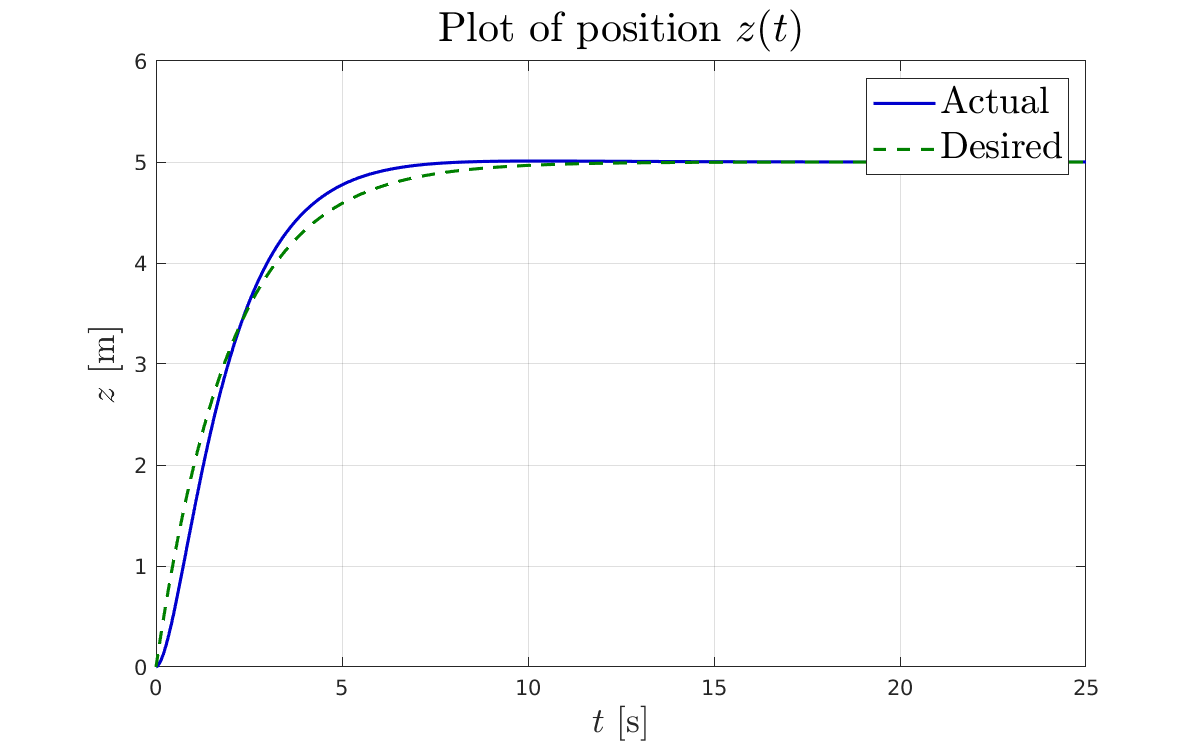
\includegraphics[width=\textwidth]{images/pid_z.png}
        \caption[Tracking in Z-axis]{Actual and desired $z$ position over time.}
        \label{fig:pid_z}
    \end{minipage}
\end{figure}

\begin{figure}[h!]
    \centering
    %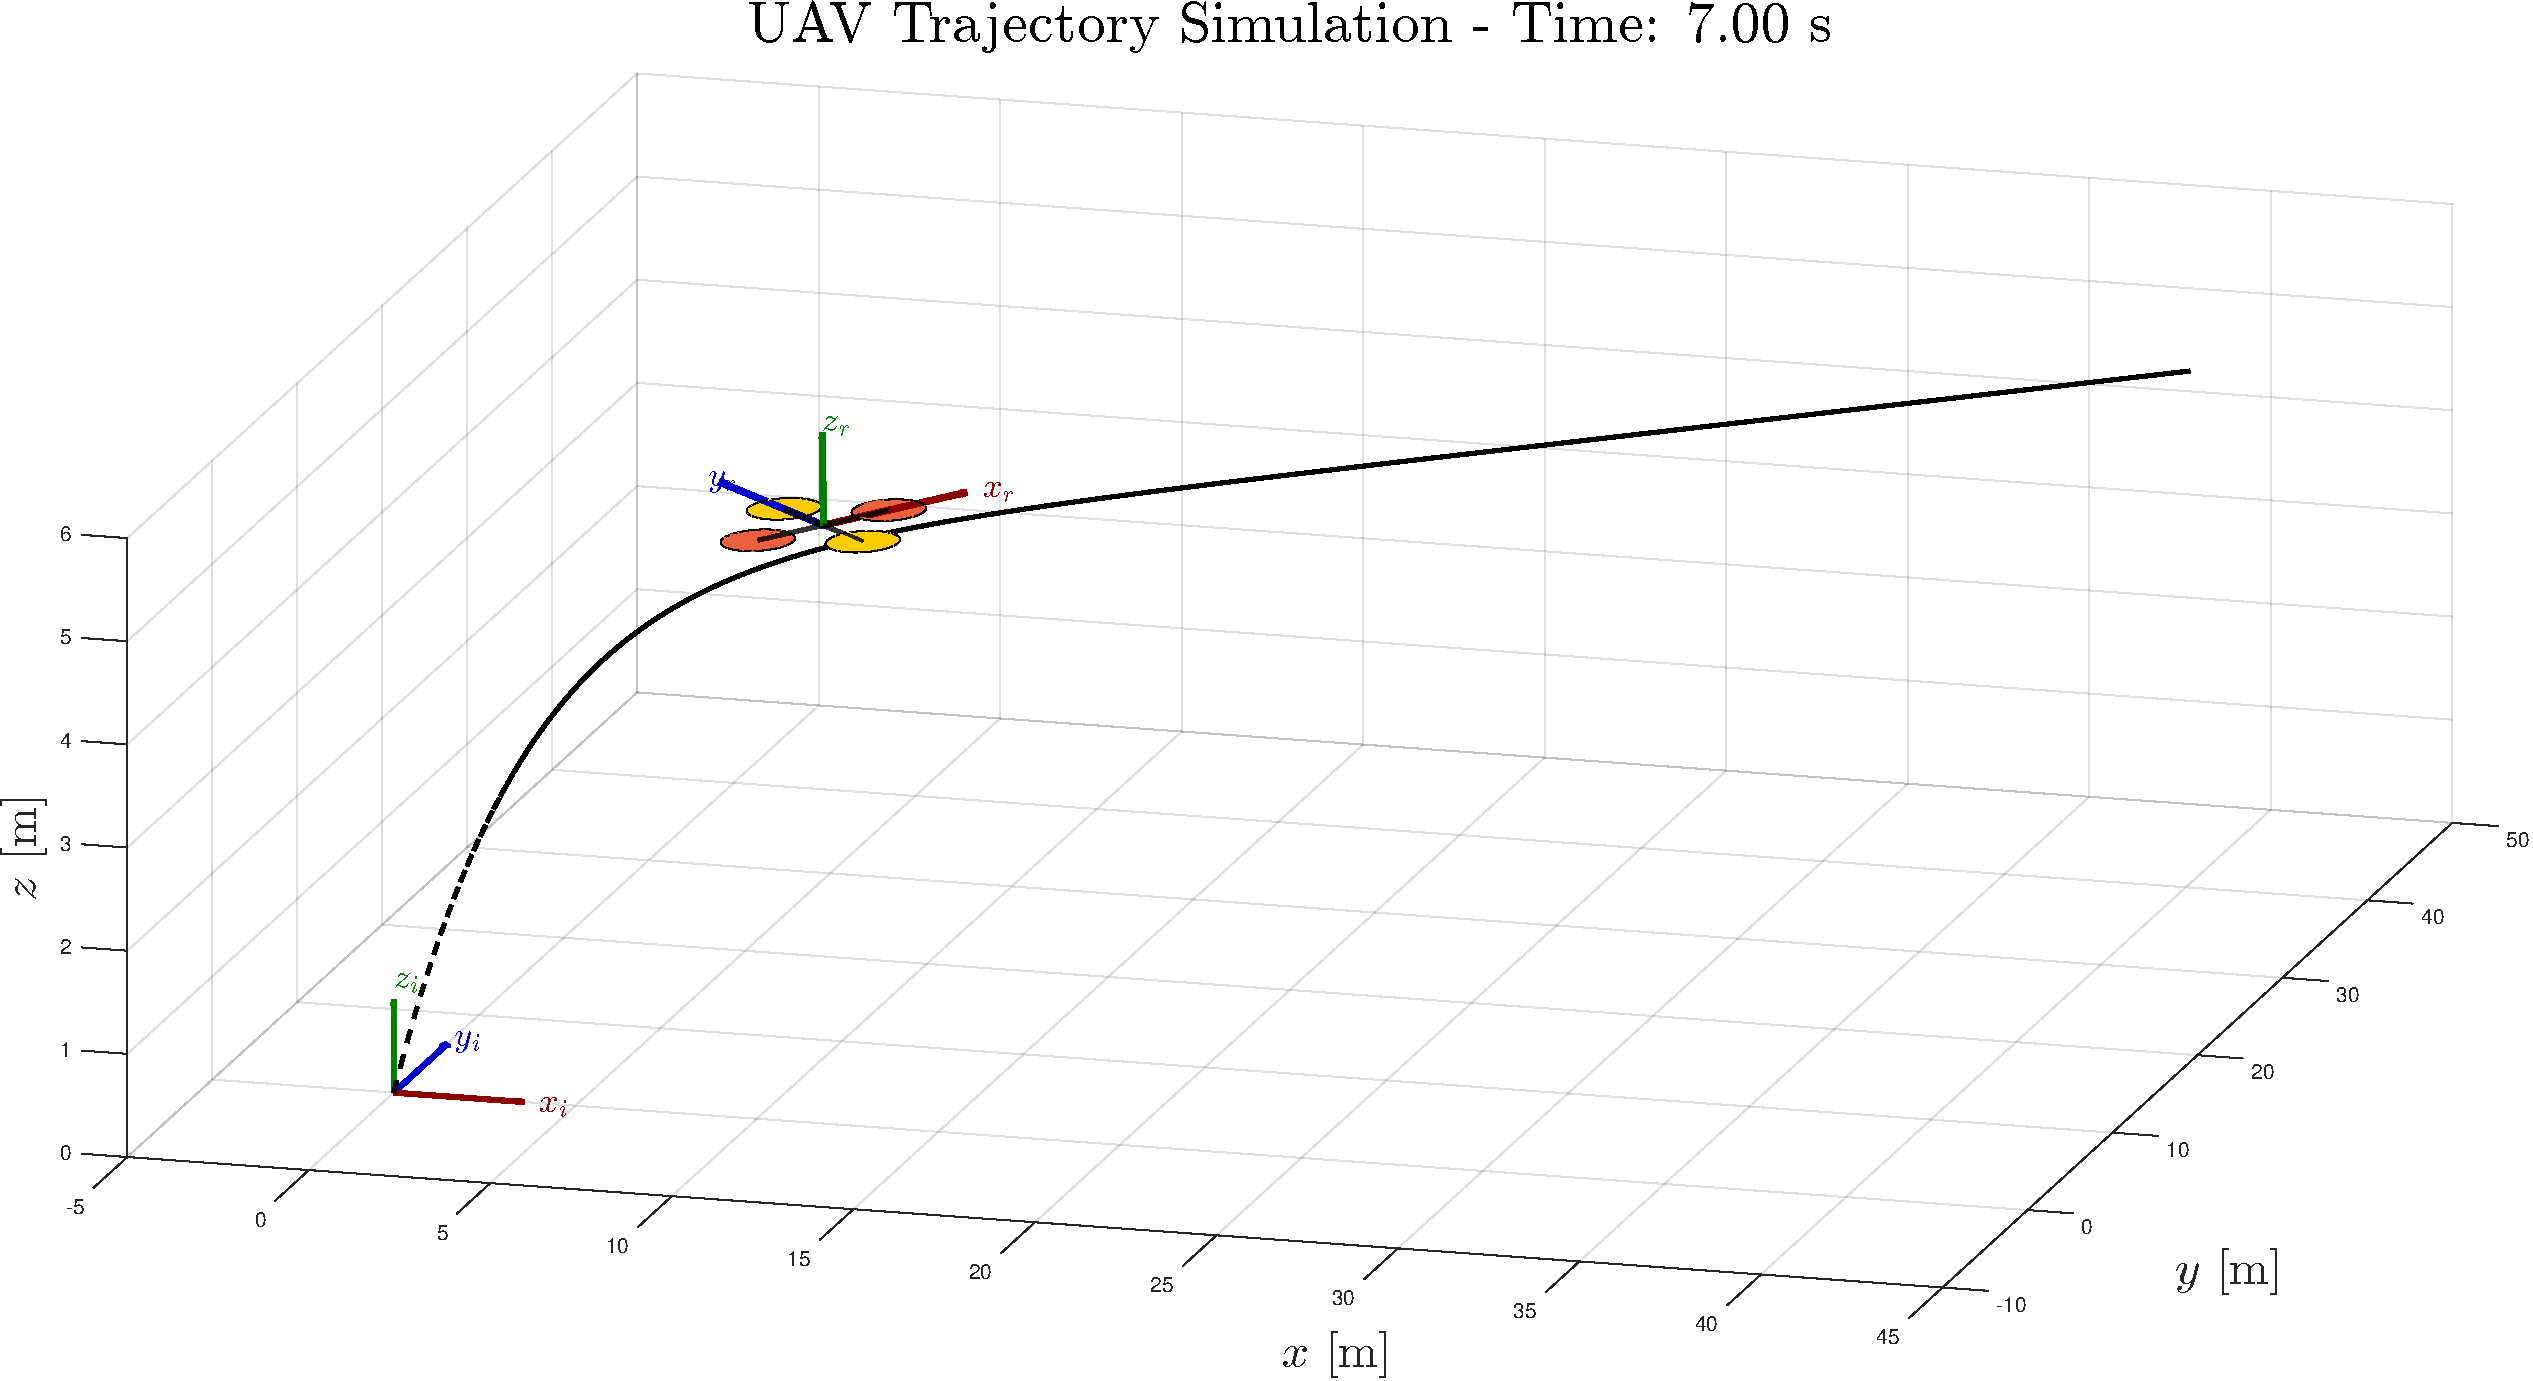
\includegraphics[width=\textwidth]{images/pid_sim.png}
    \caption[Simulation Overview]{Time instant during the simulation illustrating the system's dynamic behavior.}
    \label{fig:pid_sim}
\end{figure}

\begin{figure}[h!]
    \centering
    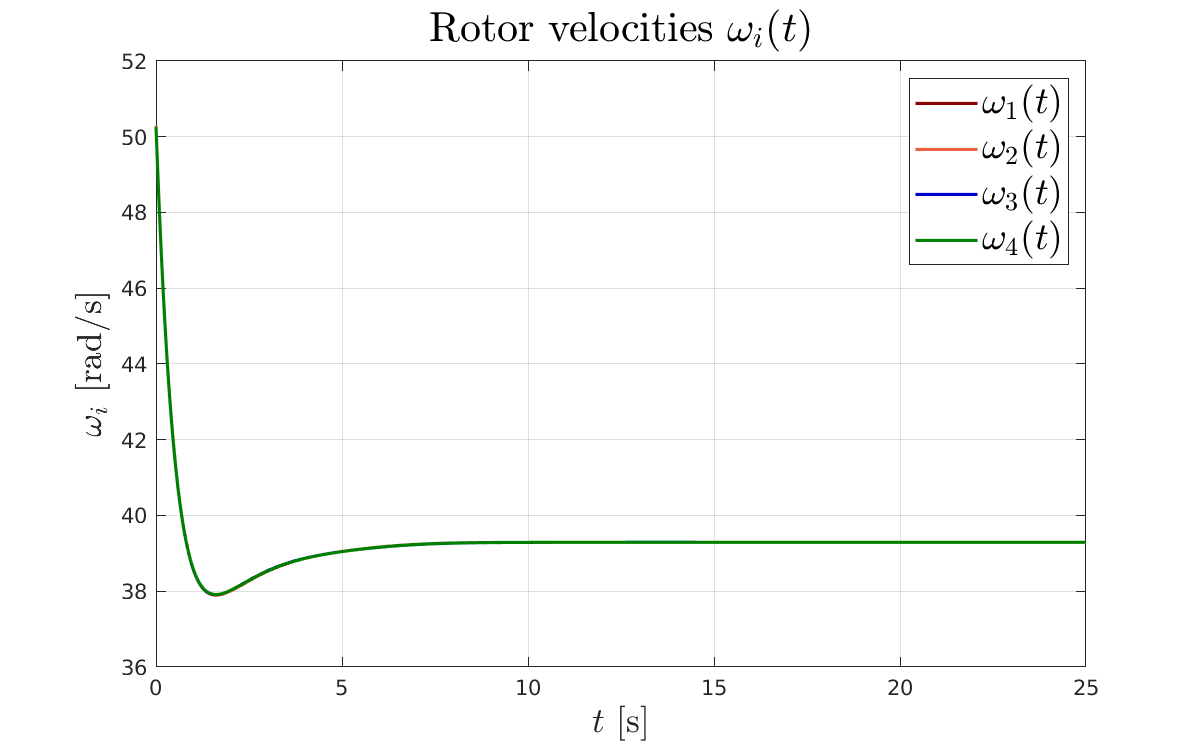
\includegraphics[width=0.49\textwidth]{images/rotor_velocities.png}
    \caption[Rotor Velocities]{Rotor velocities over time as calculated using \eqref{eq:rotor_velocities}, showing the actuation required for trajectory tracking.}
    \label{fig:rotor_velocities}
\end{figure}

\section{PSO wih Control}
\subsection{Case 1}
\subsection{Case 2}
\subsection{Case 3}

\section{Conclusions}
dire che e un euristica quindi non e sempre sicuro
+ droni ovviamnete piu facile e 
ma comunque buoni risultati in generale 
puo succedere che l algoritmo non funzioni bene a volte 
perchè i droni rimangono
attratti sempre dalle stesse sorgenti e non 
"vedono" delle altre ma questo è una cosa diciamo 
intrinseca al problema in se che stiamo affrontando.


The exclusion zone mechanism allows the swarm 
to adaptively adjust its search strategy based on the locations 
of previously detected sources, leading to faster convergence 
and improved accuracy in multi-source localization.


PUT ADVANTAGES OF DECENTRALIZED APPROACH
QUESTO È QUELLO CHE AVEVAMO SCRITTO NEL PROGETTO
Furthermore, decentralization provides improved robustness to "communication noise" by removing 
dependence on a central computation unit. This autonomy enables the system to adapt to varying 
communication conditions, such as intermittent information availability or delays, thus supporting 
continued operation in challenging environments such asmountain regions and adverse weather 
conditions, like in our scenario. While decentralized methods may exhibit slower convergence and slightly higher estimation 
errors due to partial information exchange, they remain effective and efficient in situations where 
centralized coordination is impractical or demands excessive resources.
Our algorithm favors a decentralized approach, which is useful 
in scenarios where communication between drones is not always 
possible or easy.